\section{Methods} \label{sec:methods}

\subsection{Signature of Multilevel Selection}

A fundamental characteristic of multilevel selection is in establishing conflicting incentives between short- and long-term inclusive fitness.
From the point-of-view of evolution of multicellularity, short-term increases in cell proliferation lead to long-term detriments to the capability of the multicellular organism as a whole to survive and reproduce (e.g., cancer).
Analagous split-level selective dynamics can also emerge outside the context of cooperative higher-level multicellularity.
In the context of host-parasite dynamics, traits can exhibit short-term benefits by facilitating within-host proliferation but harm the capability of the strain to infect further hosts --- e.g., due to prematurely killing the host or reduced proficiency or proclivity in escaping the host environment.

% graphics source https://docs.google.com/presentation/d/111HE56Ow0miZApHPBa18eyPAw8cdslZyBCavoWMix8E
\begin{figure}

\begin{minipage}{0.5\linewidth}
\centering
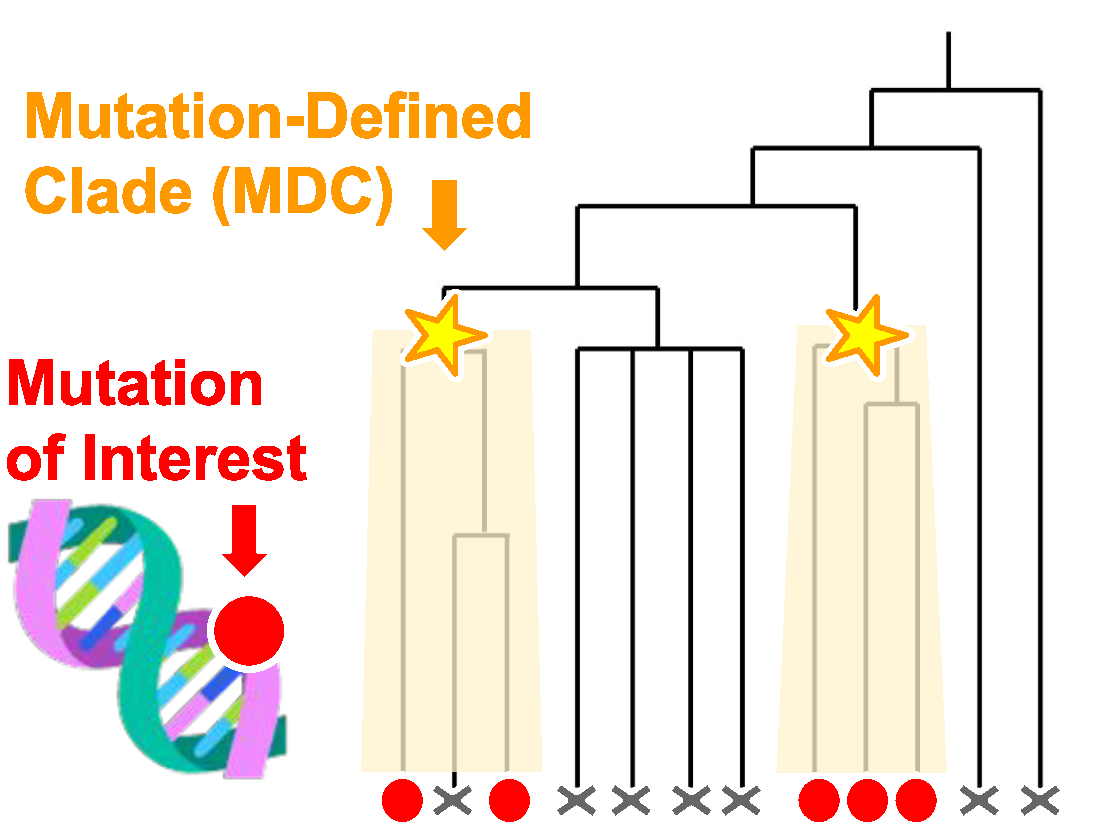
\includegraphics[width=\linewidth]{img/mls-schematic-mdc}
\subcaption{mutation-defined clades}
\label{fig:mls-schematic:mdc}
\end{minipage}%
\begin{minipage}{0.5\linewidth}
\centering
\begin{minipage}{\linewidth}
\centering
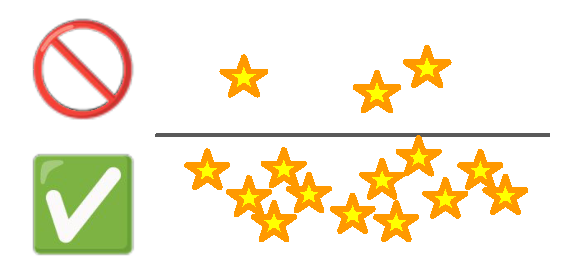
\includegraphics[width=0.8\linewidth]{img/mls-schematic-mutfreq}
\subcaption{mutation frequency}
\label{fig:mls-schematic:mutfreq}
\end{minipage}
\begin{minipage}{\linewidth}
\centering
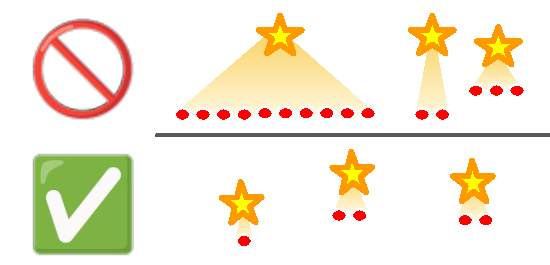
\includegraphics[width=0.8\linewidth]{img/mls-schematic-fiteffect}
\subcaption{fitness effect}
\label{fig:mls-schematic:fiteffect}
\end{minipage}
\end{minipage}

\caption{\textbf{Adapted method to screen for multilevel selection on an example mutation of interest.} a) The phylogeny for the mutation of interest. In this case, the mutation arises twice (indicated by stars), producing two mutation-defined clades (highlighted in yellow). Red circles indicate leaf taxa with the mutation. b) Mutations under MLS should be observed more often than expected by chance. c) Mutations under MLS should go on to produce smaller clades than expected by chance.}
\label{fig:mls-schematic}

\end{figure}


In the presence of multilevel selection dynamics, therefore, there exist mutations that can briefly surge in prevalence but ultimately be swept to extinction.
It is these specific genome sites that we explore how to identify in this work.
We adopt the strategy proposed by \citep{BonettiFranceschi2024phylogenetic}, wherein these sites are identified as
\begin{enumerate}
\item appearing in the population at a higher rate than expected for a random neutral mutation (given transient short-term fitness benefit), and
\item being associated with smaller, shorter-lived clades than expected for neutral mutations (due to longer-term disadvantage).
\end{enumerate}

This approach therefore requires two types of information: (1) genome sequences, so that the sets of mutations carried by different individuals in a population cab be identified and (2) phylogeny, so that lineage history outcomes may be assessed.
In biological study systems, these two types data are typically intrinsically linked due to sequence data being used as the basis to infer phylogenetic history.
However, this is not always the case in digital study systems, where phylogeny may be more readily tracked directly.

Indeed, in direct phylogeny tracking in digital systems, it is often possible to record the exact point at which a mutation originated.
Howevever, in other scenarios like biological model systems or very large-scale digital simulations, this information may not be available.
In that case, is therefore necessary to estimate the point in evolutionary where mutations held by members of a population actually arose for the first time.
\citet{BonettiFranceschi2024phylogenetic} use an \textit{ad hoc} approach accomplish this by labeling tips according to whether or not they contain a mutation and identifying inner nodes for which $\geq75\%$ of descendant tips on one daughter branch contain a mutation but $<75\%$ of nodes on the other do not contain that mutation.
The clade for which individuals have a mutation through common descent is termed as a \textit{Mutation-Defined Clade (MDC)}.
In usage in this work, we use direct tracking approaches and the term MDC instead refers to the exact point at which a mutation arises.

In sum, therefore, our goal is to identify particular genome sites for which (1) a higher quantity of MDCs are observed than expected by chance and (2) when MDCs do occur, they tend to be smaller and/or more short-lived than by chance.
(Figure \ref{fig:mls-schematic}).

In the next section, we will describe the original statistical algorithm proposed by \citet{BonettiFranceschi2024phylogenetic} for this purpose, and our proposed modifications.

\subsection{Site Screen Methodology}

One of the challenges of characterizing fitness outcomes from a phylogeny is in accounting for a myriad of possible confounding factors.
Several possible examples include: further clade history after the point at which a clade is sampled (e.g., recency bias), differences in genetic background having effects on selection (e.g., emergence of high-transmission strains that like alpha, beta, omicron etc.), time-varying environmental effects (e.g., habitat/resource availability, predation).

\citet{BonettiFranceschi2024phylogenetic} propose an elegant approach to account for these issues: compare between each MDC and its sister clade.
These clades and,
Essentially, the difference between these clades can be interpreted as differing solely in terms of the putatively-causal influence of the mutation of interest.

% graphics source https://docs.google.com/presentation/d/111HE56Ow0miZApHPBa18eyPAw8cdslZyBCavoWMix8E
\begin{figure}[htb]
\centering
\begin{minipage}{0.47\linewidth}
\centering
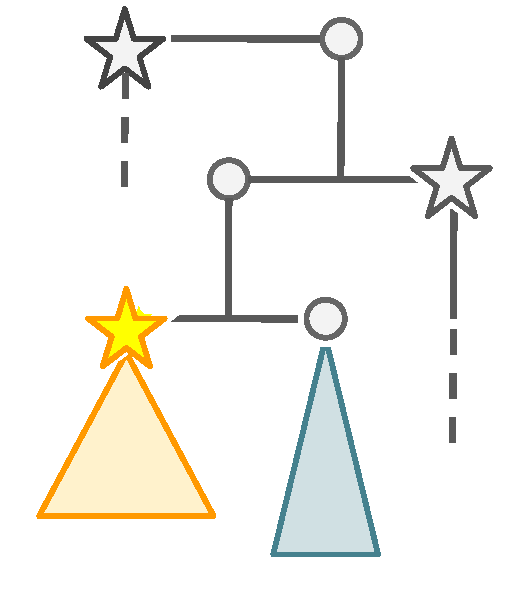
\includegraphics[width=0.7\linewidth]{img/screen-strategy-tree-balance}
\subcaption{one sister clade comparator}
\label{fig:screen-strategy:tree-balance}
\end{minipage}
~~
\begin{minipage}{0.47\linewidth}
\centering
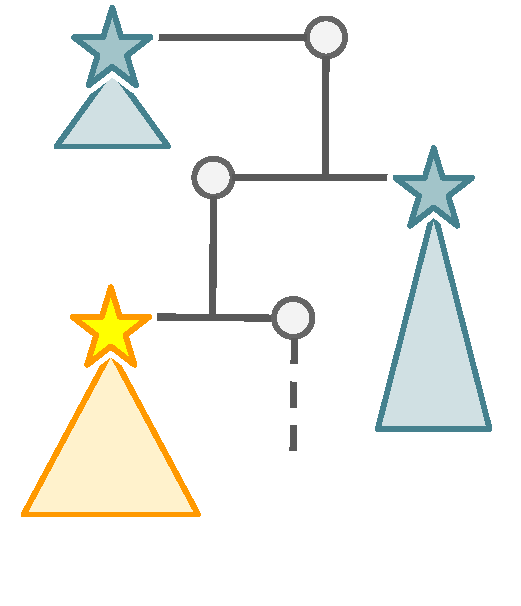
\includegraphics[width=0.7\linewidth]{img/screen-strategy-comparator}
\subcaption{multiple MDC comparators}
\label{fig:screen-strategy:window}
\end{minipage}
\vspace{-1ex}
\caption{%
\textbf{Fitness-effect screen strategies.}
\footnotesize
Yellow star indicates mutation of interest, yellow triangle indicates the clade it defines. Teal triangles indicate comparator clades. Teal stars indicate mutations defining comparator clades. Grey stars indicate mutations defining clades that are neither the focal clade nor comparator clades.
a) As proposed by \citep{BonettiFranceschi2024phylogenetic}, the focal clade is compared to its sister clade (which may or may not be mutation-defined), b) The focal clade is compared to a collection of other mutation-defined clades (MDCs).
}
\label{fig:screen-strategy}
\end{figure}


However, in adapting this approach to our \textit{in silico} study system we ended up developing an alternate approach wherein we normalize clade statistics to a broader set of selected comparators, rather than just the sister clade.
Specifically, we normalize against the pooled set of MDCs for \textit{other} mutations.
Figure \ref{fig:screen-strategy} provides a schematic comparison between the sister-clade and MDC comparator approaches.

Our motivation in diverging to develop the proposed comparator-based approach is twofold, driven by the unique characteristics of phylogenetic data from digital study systems.
First, we sought to enhance statistical power of the assay.
%TODO could show results with very small comparator groups to back up this point
This is a particular concern for \textit{in silico} agent-based model systems, due to the typically smaller populations that are feasible to instantiate compared to the vast population sizes typically exhibited by microbial and viral populations.
In particular, under the sister clade comparator approach, the statistics measured for each individual MDC are strongly influenced by the status of the comparator clade.

Another challenge associated with densely-sampled, exactly-tracked phylogenies is complicating artifacts in tree topology.
For instance, high density of short tips descended from internal nodes can introduce a bias towards comparison against these internal tips as sister clades.
Likewise, the existence of true multifurcations, which must be arbitrarily resolved in order to perfkrm binary comparisons, also further compliicates matters \citep{TODOphylotrackpy}.
Relatedly, another related useful factor of the comparator-based approach is in normalizing exclusively against other phylogeny nodes where mutations arose (e.g., incubation time, infection order, etc.).
This also accounts for possible biasing heterogeneity in the composition of internal nodes where mutations arise, whereas the sister comparator approach largely compares against non-MDC nodes.

\citet{BonettiFranceschi2024phylogenetic} apply a combination of three clade statistics to quantify empirical fitness characteristics of clades.
\begin{enumerate}
\item clade size,
\item clade duration,
\item clade growth rate.
\end{enumerate}

The first two metrics are taken as the ratio between the number of leaves contained within a clade versus its sister and the ratio of the elapsed chronological time between the estimated MDC-originating event and the extinction of its last leaf versus that for its sister, respetively.

The third metric is has a more subtle calculation and interpretation.
\citet{TODOOTHERVOLZ} suggests that the relative growth rate between two clades can be estimated by performing binary logistic regression.
In this approach, membership in clade A versus clade B is considered as a binary response variable and the predictor variable is taken as chronological time.%
\footnote{%
Logistic regressions are moderately computationally expensive to perform,
In exploratory work, we anecdotally found directionally-consistent results with orders-of-magnitude faster runtime could be achieved by applying recently-proposed fast approximations for binary logistic regression applied in \citep{TODO}.
Further investigation is warranted in this regard.
}

Due to the multiple-comparator approach pursued in this work, we adopt generalizations of clade fitness measures generalized beyond the binary measures used by \citet{BonettiFranceschi2024phylogenetic}.
For the clade size and clade duration measures, we normalize against the comparator group through a simple percentile ranking.
(Because of strong discretization effects, we take mean rank measure for tie-breaking.)
For the sake of simplicity, we omit the logistic clade growth measure from current work given that devising a generalization beyond simple binary comparison would be more involved.

% graphics source https://docs.google.com/presentation/d/111HE56Ow0miZApHPBa18eyPAw8cdslZyBCavoWMix8E
\begin{figure}
\centering
\begin{minipage}{0.47\linewidth}
\centering
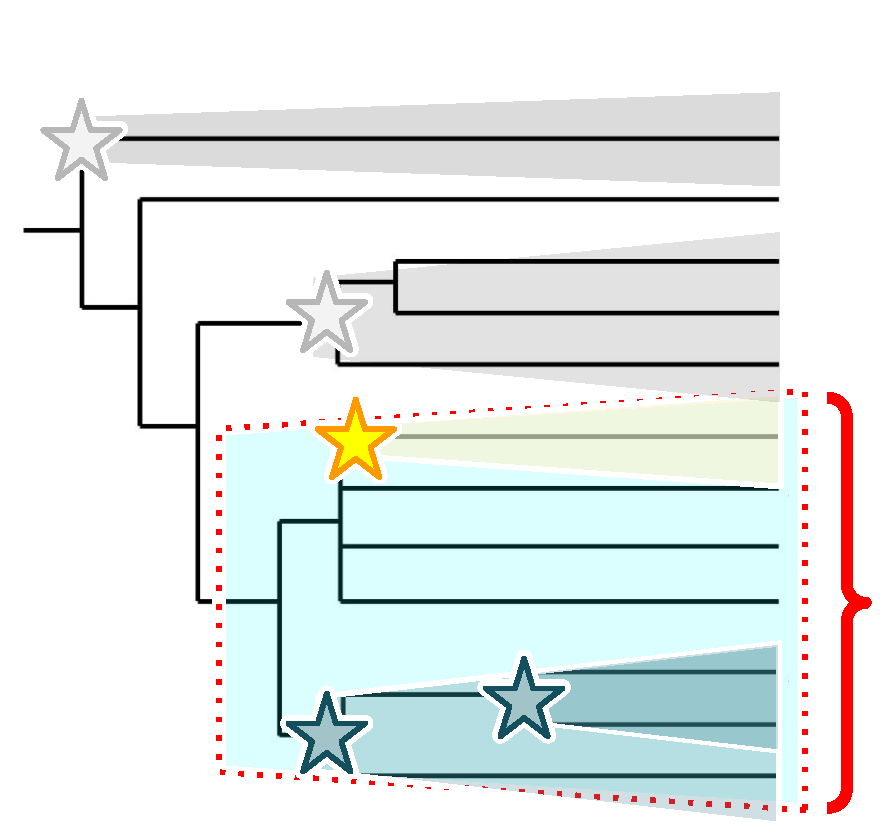
\includegraphics[height=0.75\linewidth,angle=270]{img/comparator-selection-clade}
\subcaption{phylogeny-based}
\label{fig:comparator-selection:clade}
\end{minipage}
~~
\begin{minipage}{0.47\linewidth}
\centering
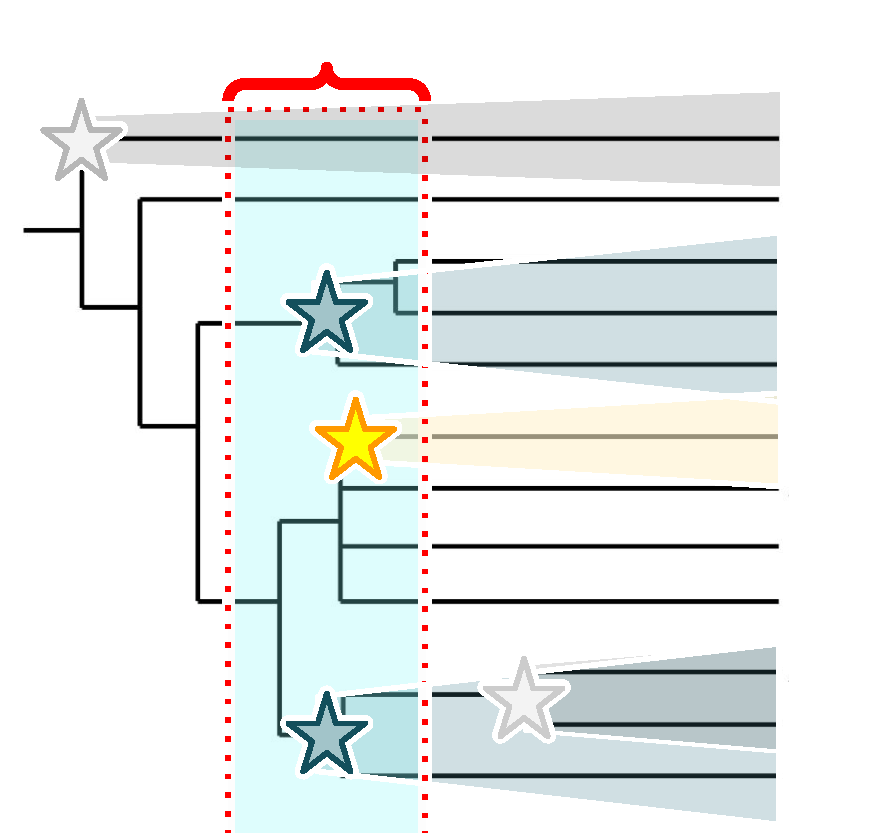
\includegraphics[height=0.75\linewidth,angle=270]{img/comparator-selection-window}
\subcaption{epoch-based}
\label{fig:comparator-selection:window}
\end{minipage}

\begin{minipage}{\linewidth}
\caption{%
\textbf{Strategies for comparator selection.}
\footnotesize Yellow star indicates mutation of interest, teal star indicates mutations defining comparator clades. Grey stars indicate mutations defining clades that are neither the focal clade nor comparator clades.
a) Comparator group is all mutation-defined subclades of a larger clade. b) Comparator group is all mutation-defined clades that originated within a specific timespan.
}
\label{fig:comparator-selection}
\end{minipage}
\vspace{-3ex}
\end{figure}


To account for confounding and biasing factors mentioned above, it is possible to fine-tune the set of comparator MDCs sampled to provide a more apples-to-apples comparison.
Figure \ref{fig:comparator-selection} summarizes the two comparator selection explored in this work.
To account for variation on account of recency-bias and on account of time-varying environmental factors, the tree may be partioned into discrete temporal ``epochs,'' and comparison limited to other MDCs occuring within the same epoch.
To account for variation on account of extrinsic genetic factors, the tree may be partitioned into a set of comparator clades.
These may be selected using domain knowledge (in this work, phylogenetic partitions are performed on the basis of WHO strain variant).
In future work, it would also be promising to explore conducting these comparisons on the basis of inferred partitions from aspects of tree topology --- for which there is exciting emerging methodologies being developed.

To perform our statistical test for deviation from expected, we perform a bootstrap test of the mean percentile ranking against the 50th approach
One notable subtlety of this approach is that comparator groups should decompose the set of available MDCs into discrete, consistent partitions.
Crucially, under this condition, sampling is guaranteed to be evenly-distributed across the percentile scale (because the percentile scale is consistently defined in terms of sampled values).
This ensures that comparing againt the 50th percentile is appropriate because that is the true group mean.

To account for intrinsic uncertainty in real-world biological data,
\citet{BonettiFranceschi2024phylogenetic} take several further quality-control steps in excluding data beyond a fixed minimum clade size threshold and excluding genome regions known to be associated with sequencing anomolies from consideration.
However --- given that we are using perfect-fidelity data from a digital model --- for the sake of simplicity and to maximize statustucak power of our datasets, we omit these adjustments.

\subsection{Test Platform: Covid-19 ABM}

% graphics source https://docs.google.com/presentation/d/111HE56Ow0miZApHPBa18eyPAw8cdslZyBCavoWMix8E
\begin{figure*}[htbp]
\begin{minipage}{0.65\linewidth}
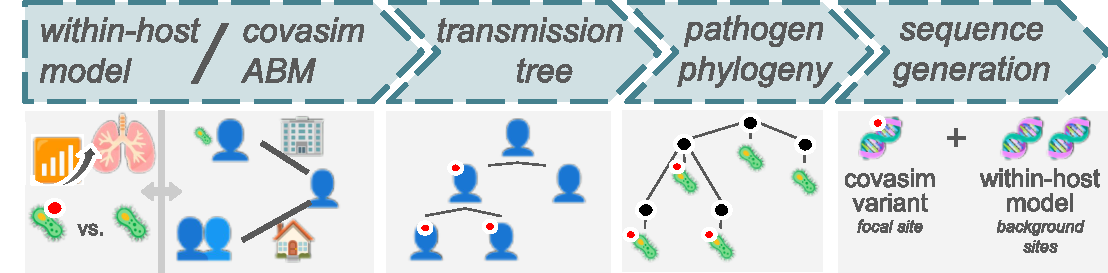
\includegraphics[width=\linewidth]{img/covasim-schematic}
\end{minipage}
\begin{minipage}{0.34\linewidth}
\caption{\textbf{Test Data Generation Pipeline.} \footnotesize Joint within-host/between-host evo-epidemiological modeling produces a sample transmission tree, then converted to a plausible ground-truth pathogen phylogeny. Accompanying strain metadata determines genetic sequence content for each viral particle.}
\label{fig:covasim-schematic}
\end{minipage}
\vspace{-3ex}
\end{figure*}


\subsubsection{Covasim Platform}

We leveraged a pre-existing agent-based epidemiological modeling platform called Covasim for this work.
This software includes features to capture a variety of aspects of relevant real-world factors, including the structure of social networks within a population (e.g., school, work), development of host immunity, and public health responses (quarantine policy, community containment efforts, etc.).

For our experiments, we used population sizes of either 200,000 or 1.2 million agents.
We simulated a 650 day window between TODO and TODO.
For the most part, we used default covasim parameter settings, although we chose a faster decay rate for host immunity to prevent extinctions of viral populations.
For simulations configured to test robustness to environmental variability, we used an existing suite of configurations emulating the timeline of vaccination rollouts and public health policies within the United Kingdom.
Experiments assumed the wildtype 2020 strain, except for multi-strain experiments which additionally incorporate extrinsic imports of alpha, beta, and gamma strains at the approximate dates where they were first observed in the course of the Covid-19 pandemic.

Although the covasim framework included capability for representing a fixed number of predefined strains arising at predetermined timepoints, in order to model the \textit{in situ} evolution of genetic traits we had to extend the existing code with a within-host evolution model, which we describe next.

\subsubsection{Within-host Model}

\subsubsection{Phylogeny Tracking}

\subsection{Treatment Conditions}

Terminology --- S: self (L0) a.k.a. within-host, G: group (L1) a.k.a transmission --- neu: neutral, ben: beneficial, del: deleterious

\begin{enumerate}
  \item Neutral Site (Sneu/Gneu) [control treatment]
  \item L0/L1-tradeoff Site (Sben/Gdel) [i.e., True TFP]
    \begin{itemize}
      \item Weak (Sben/Gdel:1\%)
      \item Moderate (Sben/Gdel:5\%)
      \item Strong (Sben/Gdel:25\%)
    \end{itemize}
  \item L0-adaptive Site (Sben/Gneu) [control treatment]
    \begin{itemize}
      \item Weak (Sben/Gneu:1\%)
      \item Moderate (Sben/Gneu:5\%)
      \item Strong (Sben/Gneu:25\%)
    \end{itemize}
\end{enumerate}


\noindent scenarios NOT consided:
\begin{itemize}
  \item pure L1-adaptive or L0/L1 adaptive sites: these will tend to sweep to fixation and are easily detected/recognized using existing methods
  \item L0-maladaptive sites: these will remain very rare, and if we can distinguish neutral sites we can distinguish these
\end{itemize}

\subsubsection{Effect Sizes}

\subsubsection{Confounding Factors}
\noindent Complicating factors not considered:
\begin{itemize}
  \item sampling bias
  \item pleiotropy/epistasis
  \item virulence (not considered/modeled directly)
\end{itemize}


\subsubsection{Simulation Outcomes}

\begin{figure*}
\centering

\begin{minipage}{0.32\linewidth}

\includegraphics[height=\linewidth, angle=90, trim={2cm 0 2.5cm 2cm}, clip]{binder/binder-2025-05-17-vanilla-treeviz.ipynb/binder/teeplots/2025-05-17-vanilla-treeviz/trt_name=sneu-gneu+viz=draw-biopyhlo-vertical+ext=.pdf}
\subcaption{Sneu/Gneu}
\label{fig:phylos-vanilla-example:sben-gneu}
\end{minipage}

\begin{minipage}{0.32\linewidth}

\includegraphics[height=\linewidth, angle=90, trim={2cm 0 2.5cm 2cm}, clip]{binder/binder-2025-05-17-vanilla-treeviz.ipynb/binder/teeplots/2025-05-17-vanilla-treeviz/trt_name=sben1-1x-gneu+viz=draw-biopyhlo-vertical+ext=.pdf}
\subcaption{Sben1.1$\times$/Gneu}
\label{fig:phylos-vanilla-example:sben1.1x-gneu}
\end{minipage}
\begin{minipage}{0.32\linewidth}

\includegraphics[height=\linewidth, angle=90, trim={2cm 0 2.5cm 2cm}, clip]{binder/binder-2025-05-17-vanilla-treeviz.ipynb/binder/teeplots/2025-05-17-vanilla-treeviz/trt_name=sben1-3x-gneu+viz=draw-biopyhlo-vertical+ext=.pdf}
\subcaption{Sben1.3$\times$/Gneu}
\label{fig:phylos-vanilla-example:sben1.3x-gneu}
\end{minipage}
\begin{minipage}{0.32\linewidth}

\includegraphics[height=\linewidth, angle=90, trim={2cm 0 2.5cm 2cm}, clip]{binder/binder-2025-05-17-vanilla-treeviz.ipynb/binder/teeplots/2025-05-17-vanilla-treeviz/trt_name=sben2x-gneu+viz=draw-biopyhlo-vertical+ext=.pdf}
\subcaption{Sben2$\times$/Gneu}
\label{fig:phylos-vanilla-example:sben2x-gneu}
\end{minipage}

\begin{minipage}{0.32\linewidth}

\includegraphics[height=\linewidth, angle=90, trim={2cm 0 2.5cm 2cm}, clip]{binder/binder-2025-05-17-vanilla-treeviz.ipynb/binder/teeplots/2025-05-17-vanilla-treeviz/trt_name=sben1-1x-gdel1-1x+viz=draw-biopyhlo-vertical+ext=.pdf}
\subcaption{Sben1.1$\times$/Gdel1.1$\times$}
\label{fig:phylos-vanilla-example:sben1.1x-gdel1.1x}
\end{minipage}
\begin{minipage}{0.32\linewidth}

\includegraphics[height=\linewidth, angle=90, trim={2cm 0 2.5cm 2cm}, clip]{binder/binder-2025-05-17-vanilla-treeviz.ipynb/binder/teeplots/2025-05-17-vanilla-treeviz/trt_name=sben1-3x-gdel1-3x+viz=draw-biopyhlo-vertical+ext=.pdf}
\subcaption{Sben1.3$\times$/Gdel1.3$\times$}
\label{fig:phylos-vanilla-example:sben1.3x-gdel1.3x}
\end{minipage}
\begin{minipage}{0.32\linewidth}

\includegraphics[height=\linewidth, angle=90, trim={2cm 0 2.5cm 2cm}, clip]{binder/binder-2025-05-17-vanilla-treeviz.ipynb/binder/teeplots/2025-05-17-vanilla-treeviz/trt_name=sben2x-gdel2x+viz=draw-biopyhlo-vertical+ext=.pdf}
\subcaption{Sben2$\times$/Gdel2$\times$}
\label{fig:phylos-vanilla-example:sben2x-gdel2x}
\end{minipage}


\caption{%
\textbf{Representative phylogenies from vanilla conditions.}
\footnotesize
For legibility, a sampled subclade from one replicate per treatment is illustrated.
Subclades sized between 500 and 750 taxa containing at least one instance of the variant of interest were chosen.
Trees are time-scaled with respect to days elapsed.
Red branches are the variant of interest.
}
\label{fig:phylos-vanilla-example}

\end{figure*}


\subsection{Software and Data Availability} \label{sec:materials}

Simulation code, configuration files, and batch scripts for this work are available via Zenodo at \url{TODO}.
Postprocessing scripts and executable notebooks for this work are hosted separately at \url{TODO}.
Data and supplemental materials are available via the Open Science Framework \url{https://osf.io/37fv8/} \citep{foster2017open}.

This project project uses data formats and tools associated with the ALife Data Standards project \citep{lalejini2019data} and benefited significantly from open-source scientific software \citep{2020SciPy-NMeth,harris2020array,reback2020pandas,mckinney-proc-scipy-2010,waskom2021seaborn,hunter2007matplotlib,moreno2023teeplot,moreno2022hstrat,kerr2021covasim,dolson2024phylotrack,franceschi2024mlscluster,huertacepas2016ete3,moreno2024apc,lam2015numba,moreno2024dendropy,cock2009biopython,demaio2022phastsim}.

% Sequence data from NCBI Virus \citep{brister2014ncbi}: wildtype \citep{wu2020new,MN908947.3}, OY320691.1 \citep{OY320691.1}, OM095211.1 \citep{OM095211.1}, OY317474.1 \citep{OY317474.1}, OY324687.1 \citep{OY324687.1}, OQ430688.1 \citep{OQ430688.1}.
